
\section{Derivadas}


Consideremos una función $f$ de variable real a valores reales y sea $\bar{x}$ un elemento fijo de su dominio. Si consideramos $x \neq \bar{x}$ en el dominio, entonces la recta secante que une $x$ con $\bar{x}$ podría verse como en la figura: 
\begin{center}
	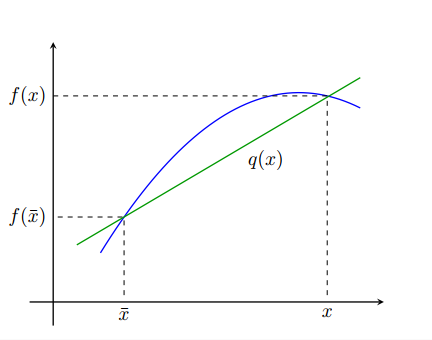
\includegraphics[scale=0.5]{figuras/capitulo1/05-derivadas/intro.png}
\end{center}
Estudiaremos el comportamiento de esta recta secante para el caso límite cuando $x \rightarrow \bar{x}$.
La noción de derivada juega un rol fundamental en economía, pues permite analizar los cambios marginales en los valores de una función. 

\textcolor{red}{Referencia: Apunte Introducción al Cálculo, semana 14; Apunte Cálculo Diferencial e Integral, semanas 1, 2 y 3.} 

\subsection{Derivadas}

Recordemos que, dada una función $f$ y $x, x_0 \in Dom(f)$ la ecuación de la recta secante que une los puntos $(x_1, f(x_1))$ con $(x_0, f(x_0))$ viene dada por: 
$$ y - y_0 = \dfrac{f(x_1) - f(x_0)}{x_1  - x_0} (x-x_0) $$ 		
Queremos estudiar la expresión anterior en el caso límite en que $x_1 \rightarrow x_0$. 
Para poder estudiar este límite, necesitamos que $x_0 \in Dom(f)$ y que $f$ esté bien definida en torno a $x_0$. 


\begin{definicion}
	\textbf{(Interior)} 
	Dado $A \subseteq \R$, diremos que $x \in int (A)$ si $\exists \delta > 0$ tal que $(x - \delta , x + \delta ) \subseteq Dom(f)$. 
\end{definicion}	

\begin{definicion}
	\textbf{(Derivada)}
	
	Sea $f: A \subseteq \R \longrightarrow \R$, diremos que $f$ es \textbf{derivable} o \textbf{diferenciable} en $x_0 \in Int(A)$ si y solo si el límite: 
	$$ \lim_{h\rightarrow 0} \dfrac{f(x_0 + h) - f(x_0)}{h} $$ 
	Existe. 
	
	En tal caso, el valor del límite se denominará derivada de $f$ en $x_0$ y se denotará por $f'(x_0)$. 
\end{definicion}

\begin{ejemplo}
	Veamos algunos ejemplos: 
	\begin{itemize}
		\item Para $f(x) = \sqrt{x}$ se tiene que $f'(4) = \frac{1}{4}$. 
		\item Para $f(x) = \sqrt[3]{x}$ no existe la derivada en $x_0 =0$. 
		\item Para la función $f(x) = |x|$, $f'(x_0) = 1$ si $x_0 > 0$, $f'(x_0) = -1$ si $x_0 < 0$ y $f'(x_0)$ no existe para $x_0 = 0$. 
	\end{itemize}
\end{ejemplo}

\begin{definicion}
	\textbf{(Función derivada)}
	Sea $f$ una función, entonces la función tal que $x \rightarrow f'(x)$ se llama \textbf{función derivada} de $f$ y se denota por $f'$. 
\end{definicion}

\begin{nota}
	El dominio de $f$ y $f'$ no necesariamente coincide: tomar por ejemplo $f(x) = | x |$. 
\end{nota}
	
	
\begin{proposicion}
	Algunas derivadas que suponemos conocidas son las siguientes: 
	\begin{itemize}
		\item $f(x) = c$, $f'(x) = 0$
		\item $f(x) = x^n$, $f'(x) = n x^{n-1}$
		\item $f(x) = \sqrt[n]{x}$, $f'(x) = \frac{1}{n} a^{1-n}$
		\item $f(x) = \ln(x)$, $f'(x) = \frac{1}{x}$
		\item $f(x) = e^x$, $f'(x) = e^x$
		\item $f(x) = x^\alpha$, $f'(x) = \alpha x^{\alpha -1}$
		\item $f(x) = sen(x)$, $f'(x) = cos(x)$
		\item $f(x) = cos(x)$, $f'(x) = - sen(x)$
	\end{itemize}
\end{proposicion}


\subsection{Álgebra de derivadas}

\begin{proposicion}
	Si $f$ y $g$ son diferenciables en $x_0$ y $\alpha \in \R$, entonces $f \pm g$, $\alpha f$, $fg$ y $f/g$ con $g(x_0) \neq 0$ son también diferenciables y además: 
	\begin{itemize}
		\item $(f\pm g))' = f' \pm g'$
		\item $(\alpha f) ' = \alpha f'$
		\item $(fg)' = f'g + f g'$
		\item $(f/g)' = \dfrac{f'g - fg'}{g^2}$
	\end{itemize}
\end{proposicion}

\begin{teorema}
	\textbf{(Regla de la cadena)}
	Sea $f$ diferenciable en $x_0$ y sea $g$ diferenciable en $y = f(x_0)$, entonces $g\circ f$ es diferenciable en $x_0$ y además se cumple que: 
	$$ (g\circ f)'(x_0) = g'(f(x_0))\cdot f'(x_0) $$ 
\end{teorema}

\begin{proposicion}
	\textbf{(Derivada de la función inversa)}
	Sea $f:[a,b] \rightarrow [c,d]$ una función monótona y biyectiva. Si $f$ es diferenciable en $x_0 \in (a,b)$ y $f'(x_0) \neq 0$, entonces $f^{-1}$ es diferenciable en $y_0 = f(x_0)$ y además: 
	$$ (f^{-1})'(y_0)) =\dfrac{1}{f'(x_0)} = \dfrac{1}{f'(f^{-1}(y_0))} $$
\end{proposicion}

\subsection{Aplicaciones}
\begin{definicion}
	\textbf{(Mínimo local)}
	Diremos que $\bar{x}$ es un \textbf{mínimo local} de la función $f$ si existe $\varepsilon > 0$ tal que: 
	$$ f(\bar{x}) \leq f(x) , \forall x \in (\bar{x}- \varepsilon , \bar{x} + \varepsilon ) $$ 
	Y de manera análoga se define la noción de máximo local. 
\end{definicion}

\begin{teorema}
	Si $\bar{x} \in (a,b)$ es un mínimo o máximo local de una función derivable $f: (a,b) \rightarrow \R$, entonces $f'(\bar{x}) = 0$
\end{teorema}

\begin{teorema}
	\textbf{(Del valor medio)}
	Sean $f, g: [a,b] \rightarrow \R$ funciones continuas en $[a,b]$ y derivables en $(a,b)$. Entonces existe $\chi \in (a,b)$ tal que: 
	$$ [f(b) - f(a)]' g(\chi) = [g(b) - g(a)]f'(\chi) $$
	En particular, si $g(x) = x$ se tiene que: 
	$$ \dfrac{f(b) - f(a)}{b - a} = f'(\chi) $$ 
\end{teorema}

\begin{center}
	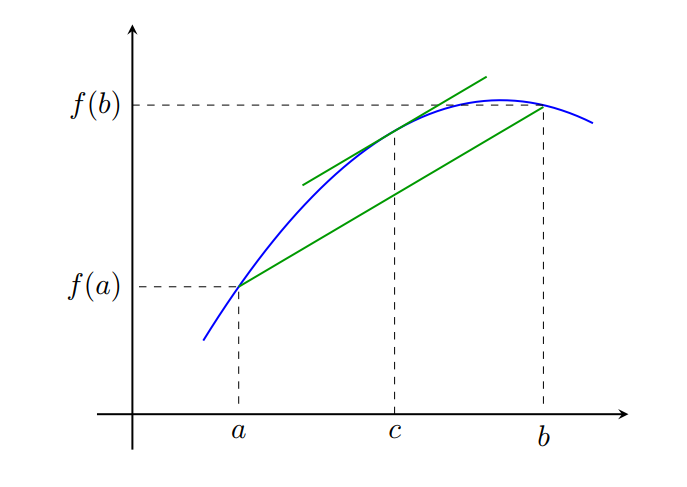
\includegraphics[scale=0.5]{figuras/capitulo1/05-derivadas/tvm.png}
\end{center}

Una consecuencia directa del TVM es la llamada \textbf{regla de L'Hopital} para el cálculo de límites de la forma $0/0/$ o $\infty /\infty$:

\begin{teorema}
	\textbf{(Regla de L'Hopital)}
	Sean $f,g:(a,b)\longrightarrow \R$ derivables en $(a,b)$ tales que: 
	$$ \lim_{x\rightarrow a^+} f(x) = \lim_{x\rightarrow a^+} g(x) = L $$ 
	Con $L = 0$ o $L = \infty$ y $g'(x) \neq 0$ para todo $x \in (a,b)$. Entonces: 
	$$ \lim_{x\rightarrow a^+} \dfrac{f(x)}{g(x)} = \lim_{x\rightarrow a^+} \dfrac{f'(x)}{g'(x)} $$ 
	Siempre que este último límite exista. 
\end{teorema}


Las derivadas nos permiten hacer conclusiones sobre la monotonía de las funciones:
\begin{proposicion}		
	Sea $f:[a,b] \longrightarrow \R$ continua en $[a,b]$ y derivable en $(a,b)$. Si $f'(x) \geq  0$ (resp. $\leq 0$) para todo $x \in (a,b)$, entonces $f$ es creciente (resp. decreciente) en $[a,b]$. Si la desigualdad es estricta, la monotonía es estricta. 
\end{proposicion}